\documentclass[10pt,letterpaper]{article}
\usepackage[english]{babel}
\usepackage[utf8]{inputenc}
\usepackage[T1]{fontenc}
\usepackage{geometry}
\usepackage{amsmath,amssymb,hyperref,xcolor,booktabs,array}
\usepackage{caption}
\usepackage{float}
\usepackage{tikz}
\usetikzlibrary{arrows.meta,positioning,fit,backgrounds}
\geometry{top=0.9in,bottom=0.9in,left=0.9in,right=0.9in}

\title{\textbf{Streaming Scene-Graph Perception with Latent Chain-of-Thought Reasoning}\\[0.2cm]
\large A real-time architecture for object-centric video understanding}
\author{Euhid Aman}
\date{(2026-06-30)}

\begin{document}
\maketitle

\section{Overview and motivation}

The goal is real-time, object-centric reasoning over a live camera stream. A monolithic
vision-language model (VLM) that ingests raw frames and emits free-text reasoning is accurate but
expensive: it re-encodes every pixel on every frame and reasons by autoregressively decoding many
natural-language tokens. We instead factor the problem into a cheap, structured \emph{perception}
front-end and a compact \emph{latent-reasoning} back-end:

\begin{enumerate}
  \item A small real-time detector extracts \textbf{object labels and boxes} from each frame.
  \item A relation module assembles those objects into a \textbf{scene graph} --- the objects and
        the relationships among them.
  \item The serialized scene graph (not the raw pixels) is handed to a reasoning model that runs
        \textbf{chain-of-thought (CoT) in a continuous latent space} rather than in words, which
        cuts the number of forward passes and therefore latency and CPU/GPU overhead.
\end{enumerate}

The design rests on three published results: single-pass real-time detection (YOLO
\cite{redmon2016}, and its open-vocabulary successor YOLO-World \cite{cheng2024}); scene-graph
generation by message passing \cite{xu2017} over Visual Genome relationships \cite{krishna2017};
and latent chain-of-thought (Coconut \cite{hao2024}), trained with the efficient
group-relative RL objective popularised by DeepSeek-R1 \cite{deepseek2025}. The remainder of this
report specifies each stage, the formulas that govern it, and why the latent back-end is the right
choice for a streaming setting.

\begin{figure}[H]
\centering
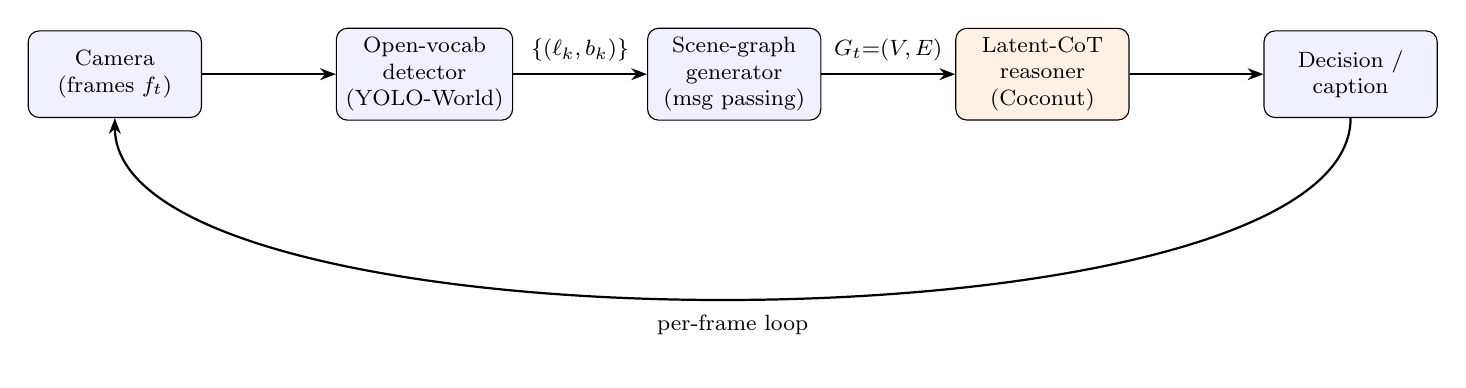
\begin{tikzpicture}[
  font=\footnotesize,
  node distance=1.7cm,
  box/.style={draw,rounded corners,minimum height=1.1cm,minimum width=2.2cm,align=center,fill=blue!6},
  rbox/.style={draw,rounded corners,minimum height=1.1cm,minimum width=2.2cm,align=center,fill=orange!10},
  arr/.style={-{Stealth[length=2mm]},thick}
]
\node[box] (cam) {Camera\\(frames $f_t$)};
\node[box,right=of cam] (det) {Open-vocab\\detector\\(YOLO-World)};
\node[box,right=of det] (sgg) {Scene-graph\\generator\\(msg passing)};
\node[rbox,right=of sgg] (llm) {Latent-CoT\\reasoner\\(Coconut)};
\node[box,right=of llm] (out) {Decision /\\caption};
\draw[arr] (cam) -- (det);
\draw[arr] (det) -- node[above=1pt]{$\{(\ell_k,b_k)\}$} (sgg);
\draw[arr] (sgg) -- node[above=1pt]{$G_t{=}(V,E)$} (llm);
\draw[arr] (llm) -- (out);
\draw[arr] (out.south) to[out=-90,in=-90,looseness=0.5]
  node[below=2pt]{per-frame loop} (cam.south);
\end{tikzpicture}
\caption{End-to-end pipeline. Perception (blue) runs per frame and emits a compact scene graph;
the reasoner (orange) consumes the graph and reasons in latent space. The loop repeats at the
camera rate.}
\end{figure}

\section{Stage 1 --- Per-frame object perception}

\textbf{Detector.} YOLO frames detection as a single regression from the full image to a fixed
grid of boxes and class scores, evaluated in one forward pass; the original network runs at
\textbf{45\,FPS} (Fast~YOLO at 155\,FPS) \cite{redmon2016}. Each grid cell predicts $B$ boxes,
each with a confidence that factorises as
\begin{equation}
\Pr(\text{Class}_i \mid \text{Object}) \cdot \Pr(\text{Object}) \cdot \mathrm{IoU}^{\text{truth}}_{\text{pred}}
  \;=\; \Pr(\text{Class}_i)\cdot \mathrm{IoU}^{\text{truth}}_{\text{pred}},
\end{equation}
so the same pass yields both localisation (the box) and the class-specific score used for
non-maximum suppression.

\textbf{Open vocabulary.} A fixed 80-class detector is too rigid for an arbitrary scene. YOLO-World
\cite{cheng2024} keeps the single-pass speed but replaces the closed classifier with a
\emph{region--text} matching head: each region embedding $e_k$ is scored against the text embedding
$t_j$ of a candidate class name (from a user-supplied vocabulary) by cosine similarity
\begin{equation}
s_{k,j} \;=\; \frac{\langle e_k,\, t_j\rangle}{\lVert e_k\rVert\,\lVert t_j\rVert},
\qquad \hat{\ell}_k = \arg\max_j s_{k,j},
\end{equation}
trained with a region-text contrastive loss. It reaches \textbf{35.4\,AP at 52\,FPS} on the
1{,}200-class LVIS benchmark \cite{cheng2024}, i.e.\ open-vocabulary recognition at real-time rate.
The stage output for frame $t$ is a set of detections $\{(\ell_k, b_k)\}_{k=1}^{n}$ with labels
$\ell_k$ and boxes $b_k\in\mathbb{R}^4$.

\section{Stage 2 --- Relationships: scene-graph generation}

Objects alone are not enough; the reasoner needs \emph{how they relate} (``gripper \textbf{above}
cup'', ``cup \textbf{on} tray''). A scene graph $G=(V,E)$ has one node $i\in V$ per detected object
and a directed edge $i\!\to\! j\in E$ per candidate relationship. Following Xu et al.\
\cite{xu2017}, the joint distribution over the graph given the image $I$ and box proposals $B_I$
factorises over nodes and ordered pairs:
\begin{equation}
\Pr(x \mid I, B_I) \;=\; \prod_{i\in V}\;\prod_{j\neq i}
   \Pr\!\big(x_i^{\text{cls}},\, x_i^{\text{bbox}},\, x_{i\to j} \,\big|\, I, B_I\big),
\end{equation}
where $x_i^{\text{cls}}$ is the object class, $x_i^{\text{bbox}}\in\mathbb{R}^4$ the box offset,
and $x_{i\to j}$ the predicate (relationship) label. Because a fixed factorisation ignores context,
the prediction is refined by \textbf{iterative message passing}: node-GRUs and edge-GRUs exchange
messages on a bipartite graph so that each object and relation is conditioned on its neighbours,
under the mean-field approximation
\begin{equation}
Q(x\mid I,B_I) = \prod_{i=1}^{n} Q\!\big(x_i^{\text{cls}},x_i^{\text{bbox}}\mid h_i\big)\,Q\!\big(h_i\mid f^{v}_i\big)
   \prod_{j\neq i} Q\!\big(x_{i\to j}\mid h_{i\to j}\big)\,Q\!\big(h_{i\to j}\mid f^{e}_{i\to j}\big),
\end{equation}
with node/edge hidden states $h_i, h_{i\to j}$ and visual features $f^v_i, f^e_{i\to j}$
\cite{xu2017}. The relationship vocabulary follows Visual Genome \cite{krishna2017}. The stage emits
$G_t$: a small symbolic structure (typically tens of triples \texttt{(subject, predicate, object)}),
orders of magnitude cheaper to carry forward than the frame itself.

\paragraph{Streaming.} Stages 1--2 run on every frame $f_t$, producing a \emph{temporal stream} of
scene graphs $G_1, G_2, \dots$. Only the \emph{delta} between consecutive graphs (objects that
appear, disappear, or change relation) needs to be fed to the reasoner, keeping the per-frame
payload small and bounded.

\section{Stage 3 --- Latent chain-of-thought reasoning}

The serialized graph $G_t$ is the prompt for a reasoning model. Standard chain-of-thought would
have the model \emph{write out} its reasoning as natural-language tokens before answering --- which
is exactly the cost we want to avoid in a per-frame loop, since each token is one transformer
forward pass.

\textbf{Latent reasoning (Coconut).} Coconut \cite{hao2024} keeps the reasoning but moves it out of
the vocabulary. In ordinary language mode the model uses input embeddings
$E_t = [e(x_1), e(x_2), \dots, e(x_t)]$, hidden states $H_t\in\mathbb{R}^{t\times d}$ with
$h_t = H_t[t,:]$, and predicts the next token by
\begin{equation}
\mathcal{M}(x_{t+1}\mid x_{\le t}) = \mathrm{softmax}(W h_t).
\end{equation}
In \emph{latent mode}, the last hidden state is fed straight back in as the next input embedding ---
bypassing the language-model head and the sampling step entirely:
\begin{equation}
E_t = \big[\,e(x_1),\dots,e(x_i),\; \underbrace{h_i, h_{i+1}, \dots, h_{t-1}}_{\text{continuous thoughts}}\,\big].
\end{equation}
Each ``continuous thought'' $h_{\bullet}$ carries the reasoning state in $\mathbb{R}^d$ without ever
being rendered as words, so a chain of reasoning costs a handful of forward passes instead of dozens
of decoded tokens.

\textbf{Why this helps here (with honest numbers).} On GSM8k arithmetic, Coconut trades a little
accuracy for far fewer tokens (34.1\% at \textbf{8.2} tokens vs.\ CoT's 42.9\% at 25.0 tokens). But
on \emph{planning- and search-heavy} reasoning --- ProsQA --- it is both \emph{more accurate and
much cheaper}: \textbf{97.0\% at 14.2} tokens vs.\ CoT's 77.5\% at 49.4 tokens \cite{hao2024}.
Relational reasoning over a scene graph (which object to act on, in what order, given the
constraints among them) is closer to the planning regime than to free-form arithmetic, so the
latent back-end is well matched: it is the case where latent CoT \emph{wins outright}.

\textbf{Efficiency model.} Let the reasoner cost $\tau$ per forward pass and take $n$ steps, so
reasoning latency is $\ell_r \approx n\tau$. In a pipelined stream where perception and reasoning
overlap, the sustainable frame rate is bounded by the slowest stage,
\begin{equation}
f_{\max} = \frac{1}{\max(\ell_p,\ \ell_r)}, \qquad \ell_p = \ell_{\text{detect}} + \ell_{\text{sgg}} .
\end{equation}
Replacing decoded tokens ($n_{\text{cot}}$) with continuous thoughts ($n_{\text{lat}}$) shrinks the
reasoning term by the token-compression ratio
\begin{equation}
S = \frac{n_{\text{cot}}}{n_{\text{lat}}} \approx \frac{25.0}{8.2}\approx 3.0\ \text{(GSM8k)}
   \quad\text{to}\quad \frac{49.4}{14.2}\approx 3.5\ \text{(ProsQA)},
\end{equation}
i.e.\ a $\sim$3--3.5$\times$ drop in reasoning forward passes (and the associated CPU/GPU work and
energy), with no extra cost on the perception side. When $\ell_r$ was the bottleneck, $f_{\max}$
rises by roughly $S$.

\textbf{Training the latent reasoner efficiently.} Coconut is trained by a curriculum that
progressively replaces language reasoning steps with continuous thoughts \cite{hao2024}. To make
the \emph{reasoning policy} itself strong without a costly value network, the model is post-trained
with Group Relative Policy Optimization (GRPO), the algorithm behind DeepSeek-R1
\cite{deepseek2025}. GRPO drops the critic and estimates the baseline from a \emph{group} of $G$
sampled answers per prompt:
\begin{equation}
A_i = \frac{r_i - \mathrm{mean}(\{r_1,\dots,r_G\})}{\mathrm{std}(\{r_1,\dots,r_G\})},
\end{equation}
\begin{equation}
\mathcal{J}_{\text{GRPO}}(\theta) = \mathbb{E}\!\left[\frac{1}{G}\sum_{i=1}^{G}
  \min\!\Big(\rho_i A_i,\ \mathrm{clip}(\rho_i, 1-\varepsilon, 1+\varepsilon)A_i\Big)
  - \beta\,\mathbb{D}_{\text{KL}}\!\big(\pi_\theta \,\Vert\, \pi_{\text{ref}}\big)\right],
\quad \rho_i = \frac{\pi_\theta(o_i\mid q)}{\pi_{\theta_{\text{old}}}(o_i\mid q)},
\end{equation}
with a rule-based reward (correctness + output format) rather than a learned reward model
\cite{deepseek2025}. Because there is no critic and no reward model, RL training memory roughly
halves --- the same efficiency philosophy the inference-time latent CoT follows.

\section{Putting it together: per-frame procedure}

\begin{table}[H]
\centering
\caption{Per-frame loop. Steps 1--2 are the cheap structured front-end; step 3 is the latent
reasoner; only the graph delta crosses the boundary.}
\begin{tabular}{rp{12.6cm}}
\toprule
\# & action \\
\midrule
1 & Detect objects in frame $f_t$ with the open-vocab detector $\to \{(\ell_k,b_k)\}$ (Eq.~1--2). \\
2 & Build/refine the scene graph $G_t=(V,E)$ by message passing (Eq.~3--4); diff against $G_{t-1}$. \\
3 & Serialize the graph delta; run $m$ continuous thoughts (Eq.~6--7) then decode a short answer. \\
4 & Emit the decision/caption; advance to $f_{t+1}$. Stages pipeline, so $f_{\max}=1/\max(\ell_p,\ell_r)$. \\
\bottomrule
\end{tabular}
\end{table}

\textbf{Design rationale, in one line each.} \emph{Detector small and single-pass} so perception
keeps up with the camera (Eq.~1, 45--52\,FPS). \emph{Open-vocabulary} so the system is not tied to
a fixed class list (Eq.~2). \emph{Explicit relationships} so the reasoner sees structure, not
pixels (Eq.~3--4). \emph{Latent CoT} so reasoning costs $\sim$3$\times$ fewer forward passes and, on
planning-style tasks, is also \emph{more} accurate (Eq.~6--8). \emph{GRPO training} so the reasoning
policy is learned without an expensive critic or reward model (Eq.~9--10).

\section{Limitations and honest caveats}

\begin{itemize}
  \item \textbf{Error propagation.} The reasoner only sees what the detector and SGG report; a
        missed object or wrong predicate cannot be recovered downstream. Perception recall is the
        ceiling on the whole system.
  \item \textbf{Latent CoT is not a free lunch.} On pure arithmetic (GSM8k) Coconut is \emph{less}
        accurate than written CoT \cite{hao2024}; its advantage is specific to planning/relational
        reasoning and to latency-bound deployments. We adopt it because scene-graph reasoning is in
        that favourable regime, not as a universal replacement.
  \item \textbf{Scene-graph generation is itself a hard, open problem} --- long-tailed predicate
        distributions on Visual Genome \cite{krishna2017} mean rare relationships are recognised
        poorly; the message-passing refinement \cite{xu2017} mitigates but does not solve this.
  \item \textbf{Interpretability trade-off.} Continuous thoughts are not human-readable by
        construction, so the reasoning trace cannot be inspected as text --- a real cost for
        debugging and safety auditing relative to natural-language CoT.
\end{itemize}

\begin{thebibliography}{9}
\bibitem{redmon2016} J.~Redmon, S.~Divvala, R.~Girshick, A.~Farhadi.
  \emph{You Only Look Once: Unified, Real-Time Object Detection.} CVPR 2016. arXiv:1506.02640.
\bibitem{cheng2024} T.~Cheng, L.~Song, Y.~Ge, W.~Liu, X.~Wang, Y.~Shan.
  \emph{YOLO-World: Real-Time Open-Vocabulary Object Detection.} CVPR 2024. arXiv:2401.17270.
\bibitem{xu2017} D.~Xu, Y.~Zhu, C.~B.~Choy, L.~Fei-Fei.
  \emph{Scene Graph Generation by Iterative Message Passing.} CVPR 2017. arXiv:1701.02426.
\bibitem{krishna2017} R.~Krishna et al.
  \emph{Visual Genome: Connecting Language and Vision Using Crowdsourced Dense Image Annotations.}
  IJCV 2017.
\bibitem{hao2024} S.~Hao, S.~Sukhbaatar, D.~Su, X.~Li, Z.~Hu, J.~Weston, Y.~Tian.
  \emph{Training Large Language Models to Reason in a Continuous Latent Space (Coconut).}
  arXiv:2412.06769, 2024.
\bibitem{deepseek2025} DeepSeek-AI.
  \emph{DeepSeek-R1: Incentivizing Reasoning Capability in LLMs via Reinforcement Learning.}
  arXiv:2501.12948, 2025.
\end{thebibliography}

\end{document}
